\documentclass[a4paper,11pt,noarxiv]{quantumarticle}

% ---------------------------------------------------------------------------
%  FOURTH DRAFT -- 2026-10-16 (quantumarticle; main text + Supplemental Material)
%  Lattice refinement + rodeo algorithm on the Hubbard model (paper III),
%  written along the lines of paper I (paper/eigenq_pairing.tex): a validated
%  reference implementation, a matched-accuracy benchmark at eight and sixteen
%  sites, and the transferable results.  Every number traces to an output of
%  notebooks/ResolutionRefHubbard.ipynb (built by scripts/build_notebook_hubbard.py
%  from src/pairinglib/hubbard.py); figures are figs/fig1-12.png extracted from it
%  (make figures-hubbard).  The Supplemental Material is eigenq_hubbard_supp.tex
%  (xr against this file's .aux).  Earlier drafts: eigenq_hubbard_v{1,2,3}_backup.tex
%  (v3 = the RevTeX/PRC third draft of 2026-10-15).  US spelling throughout.
%  \todo{...} marks what is still open.
% ---------------------------------------------------------------------------

\usepackage[utf8]{inputenc}
\usepackage[T1]{fontenc}
\usepackage{amsmath,amssymb}
\usepackage{physics}
\usepackage{graphicx}
\usepackage{booktabs}
\usepackage{xcolor}
\usepackage{hyperref}

\newcommand{\todo}[1]{\textcolor{red}{[#1]}}
\newcommand{\Hlow}{H_{\mathrm{low}}}
\newcommand{\Hhigh}{H_{\mathrm{high}}}
\newcommand{\Eobj}{E_{\mathrm{obj}}}
\newcommand{\Deff}{\Delta_{\mathrm{eff}}}
\newcommand{\SM}{Supplemental Material~\cite{SM}}

\begin{document}

\title{Lattice refinement followed by the rodeo algorithm: a gate-level
benchmark of eigenstate-preparation routes on the Hubbard chain}

\author{Scott Bogner}
\affiliation{Facility for Rare Isotope Beams and Department of Physics and Astronomy, Michigan State University, East Lansing, MI 48824, USA}
\author{Cecilie Glittum}
\affiliation{Department of Physics, University of Oslo, N-0316 Oslo, Norway}
\author{Heiko Hergert}
\affiliation{Facility for Rare Isotope Beams and Department of Physics and Astronomy, Michigan State University, East Lansing, MI 48824, USA}
\author{Morten Hjorth-Jensen}
\email{mhjensen@uio.no}
\affiliation{Department of Physics, University of Oslo, N-0316 Oslo, Norway}
\author{Gunnar Lange}
\affiliation{Department of Physics, University of Oslo, N-0316 Oslo, Norway}
\author{Ryan LaRose}
\affiliation{Department of Computational Mathematics, Science and Engineering and Facility for Rare Isotope Beams, Michigan State University, East Lansing, MI 48824, USA}
\author{Dean Lee}
\affiliation{Facility for Rare Isotope Beams and Department of Physics and Astronomy, Michigan State University, East Lansing, MI 48824, USA}
\author{Francesco Pietro Massel}
\affiliation{Department of Science and Industry Systems, University of South-Eastern Norway, N-3616 Kongsberg, Norway}
\affiliation{Department of Physics, University of Oslo, N-0316 Oslo, Norway}
\author{Jean Paul Sadia}
\affiliation{Department of Computational Mathematics, Science, and Engineering, Michigan State University, East Lansing, MI 48823, USA}
\affiliation{Center for Quantum Computing, Science, and Engineering, Michigan State University, East Lansing, MI 48823, USA}

\maketitle

\begin{abstract}
Resolution refinement transports an eigenstate adiabatically from a coarse
to a fine model space along a shift-controlled, gapped path; followed by the
rodeo algorithm, a projective energy filter, it is a route to high-fidelity
eigenstates that needs neither a classical optimizer nor training
measurements.  We implement the lattice version of this pipeline, in which
every coarse site is resolved into a block of fine sites, for the Hubbard
chain refined from four to eight and from eight to sixteen sites and for the
$2\times2\to4\times4$ plaquette, with every stage compiled to rotations and
CNOTs and validated against exact diagonalization in the conserved
$(N_\uparrow,N_\downarrow)$ sector.  Three structural results carry beyond
the model.  The Galerkin coarse Hamiltonian is itself a Hubbard model with
$(t,U)\to(t/2,U/2)$ in one dimension, so the hierarchy is self-similar and
can start from the filled dimer, a single basis state.  The path conserves
total spin and the lattice symmetry, so the transport is governed by the
lowest excitation in the symmetry sector of the target, $\Deff$, which stays
of order $t$ while the sector gap collapses to $0.05t$; the refinement time
is flat in $U$ and in size, $\Deff$ is the right filter width, and a coarse
state with the wrong quantum numbers cannot be refined at all.  And the
cost of a fixed-step digital filter scales as $1/\Deff$ per cycle with an
accuracy floor set by the step.  The benchmark is then run on equal terms:
the same Trotterized filter is applied to the prolonged and refined states,
to an ordinary adiabatic ramp from the free-fermion determinant, and to
single-layer, pruned and adaptively grown (ADAPT-VQE) unitary coupled-cluster
states, and the routes are compared by ground-state infidelity against CNOTs
per accepted preparation.  At sixteen qubits the ramp is the cheapest route
at every target, by a factor three over the pruned ansatz and sixteen over
the projector path, whose cost is the coarse term conditioned on all
antibonding qubits.  At thirty-two qubits the premise changes: the coarse eigenstate starts
ahead of the determinant, the ramp needs twice the time to keep up, the
single-layer ansatz has lost two orders of magnitude, and every filter
cycle costs $2\times10^5$ CNOTs.  There the two-local refinement path ties
with the ramp at every target from $3\times10^{-3}$ down, the projector
path reaches $10^{-3}$ within a factor two of it instead of sixteen, and the cost of every route is set
by the filter cycles it still needs --- which is why the refinement path,
whose transport delivers the best unfiltered input, is the one worth
compiling without its conditioned coarse term.
\end{abstract}

% ===========================================================================
\section{Introduction}
\label{sec:intro}
% ===========================================================================
Preparing an eigenstate of a many-body Hamiltonian on a quantum computer is
the step that every subsequent measurement of a correlated system depends
on, and the standard routes each face an obstacle at scale: variational
preparation pays for a classical optimization loop and is capped by its
ansatz~\cite{Peruzzo2014,McClean2018}, adiabatic preparation pays for the
inverse gap along its path~\cite{Albash2018}, and projective filters ---
phase estimation, polynomial filters, the rodeo
algorithm~\cite{Choi2021,Qian2024} --- pay $1/p$ for an input of overlap $p$
with the target.  \emph{Resolution refinement}~\cite{Bogner2026} was
proposed to supply the filter with a good input without an optimizer: an
eigenstate of a coarse (low-resolution) Hamiltonian is lifted by a
prolongation operator into a finer model space and transported
adiabatically along a path that stays gapped because refinement changes the
low-energy spectrum only mildly.  In Ref.~\cite{EigenQPairing2026} (paper I
below) we implemented this chain --- prepare a coarse eigenstate, prolong
and refine for a time $T$, filter with the rodeo algorithm --- at the gate
level for a hierarchy of single-particle bases of the pairing Hamiltonian,
and benchmarked it on equal terms against the same filter applied to
cheaper inputs.  The verdict there was sober: at eight and sixteen qubits an
ordinary adiabatic ramp from the Hartree--Fock determinant reached every
target accuracy at a fraction of the cost, and an adaptively grown
variational ansatz undercut all filtered routes.  The case for the
refinement stage rested on its freedom from optimization and on coarse
eigenstates that are better starts than the determinant --- a regime the
pairing hierarchy did not exercise.

The present paper carries the same pipeline, the same benchmarks and the
same cost accounting to the Hubbard model~\cite{Hubbard1963,Arovas2022},
\begin{equation}
  H=-\sum_{\langle ij\rangle\sigma}t_{ij}\big(c^\dagger_{i\sigma}c_{j\sigma}+\mathrm{h.c.}\big)
   +U\sum_i n_{i\uparrow}n_{i\downarrow},
  \label{eq:hubbard}
\end{equation}
for three reasons.  The Hubbard model is the canonical strongly correlated
fermion problem and the most frequently used benchmark for the quantum
simulation of fermions~\cite{Wecker2015,Cade2020,Cai2020,Stanisic2022}, with
the one-body hopping channel that the pairing model lacks.  It is the setting
for which resolution refinement was proposed~\cite{Bogner2026}: a
\emph{lattice} refinement in which every coarse site is resolved into a block
of fine sites, the prolongation is a product of Givens rotations, and the fine
lattice is the natural discretization of a continuum problem.  And it is not
exactly solvable in general, so the exact-diagonalization (ED) reference that
anchored every number of paper I must be produced numerically; we keep that
discipline and benchmark every stage against ED in the conserved
$(N_\uparrow,N_\downarrow)$ sector, up to the $14\,400$-dimensional sectors of
the sixteen-site chain and the $4\times4$ plaquette.

Relative to the proposal of Ref.~\cite{Bogner2026}, the rodeo
literature~\cite{Choi2021,Qian2024,Cohen2023,BeeLindgren2022} and the related
schemes that build large systems from solved pieces --- the hierarchical
fusion method~\cite{Patkowski2025fusion} and
nucleation~\cite{Sadia2026}, which grows the domain at fixed resolution ---
this work contributes three things.  (a) A \emph{reference implementation}
of lattice refinement: the block prolongation, the Galerkin coarse model in
closed form, two refinement paths (a shift-controlled projector path and a
two-local un-dimerization path), the Trotterized refinement and the
Trotterized controlled evolution of the filter, all compiled to rotations
and CNOTs, validated against ED at sixteen and at thirty-two qubits and
reproducible from one executable notebook~\cite{Code}.  (b) A
\emph{benchmark on equal terms}: the refinement-plus-filter chain is
compared with the same filter applied to the unrefined prolonged state, to
the free-fermion determinant, to an ordinary adiabatic ramp that switches
on $U$ from it, and to the single-layer, the pruned and the adaptively grown
(ADAPT-VQE~\cite{Grimsley2019}) unitary coupled-cluster states, with the
ground-state infidelity as the common observable, matched evolution
accuracy, a CNOT budget per accepted preparation, and the minimum cost at a
given target --- at eight sites (sixteen qubits) and, for the first time for
this pipeline, at sixteen sites (thirty-two qubits), where the free-fermion
input has begun to degrade.  (c) \emph{Three results that transfer}: the
self-similarity of the Galerkin hierarchy, which lets the chain of
refinements start from a single basis state; the identification of the
symmetry-protected gap $\Deff$ as the quantity that controls both the
refinement time and the filter width, together with the diagnostics that
expose a coarse state that cannot be refined; and the scaling of the
fixed-step digital filter --- cost per cycle $\propto1/\Deff$, accuracy floor
set by the step --- which decides, at every size, whether an input that is
cheaper but worse can be rescued by cycles.

The outcome of (b) is stated plainly.  At sixteen qubits ($U=4t$) the
ordinary adiabatic ramp from the free-fermion determinant is the cheapest
route to every target accuracy: $1.9\times10^4$, $4.0\times10^4$ and
$9.1\times10^4$ CNOTs for infidelities $10^{-3}$, $3\times10^{-4}$ and
$10^{-4}$, against three times more for the pruned 98-parameter ansatz,
four to seven times more for the two-local refinement path and sixteen
times more for the projector path, almost entirely in the coarse term
conditioned on all antibonding qubits.  The reason is specific to the size:
the determinant has the same overlap with the target and the same $\Deff$
as the prolonged coarse eigenstate.  At thirty-two qubits this is no longer
so: the prolonged coarse ground state starts at $p_0=0.87$ against $0.72$
for the determinant, the ramp needs $T=32/t$ instead of $16/t$, the
single-layer ansatz has lost two orders of magnitude and an adaptively
grown ansatz of two hundred operators barely reaches $10^{-2}$.  The ramp
remains the cheapest route, but the two-local refinement path now ties with
it within the sampling error at every target from $3\times10^{-3}$ down
($3.2$ against $3.0\times10^5$ CNOTs at $3\times10^{-3}$, $8.1$ against
$7.9\times10^5$ at $10^{-3}$), the variational routes cost $1.3$--$1.9$
times more, and the
projector path, which delivers the best unfiltered input, costs $1.6$--$1.9$
times more at the two tightest targets instead of sixteen.  At this size
the cost of every route is dominated by the filter cycles it still needs,
each worth $2\times10^5$ CNOTs, so what decides the comparison is how close
to the target the input starts --- and that is the quantity the refinement
stage controls.

The paper follows the structure of paper I.  Section~\ref{sec:model} fixes
the model, the sector encoding, the ED reference and the symmetry
diagnostics; Sec.~\ref{sec:pipeline} defines the lattice prolongation, the
Galerkin coarse Hamiltonian, the two paths, the filter and the comparators;
Sec.~\ref{sec:results} reports the sector-exact results, including the
symmetry protection and the wrong-sector plaquette; Sec.~\ref{sec:circuits}
gives the circuits and the matched comparison at eight sites;
Sec.~\ref{sec:large} takes the chain $8\to16$ to the circuit level; and
Sec.~\ref{sec:discussion} discusses what transfers.  The \SM{} collects the
verification material: the adiabatic bound and the response norm of the
path, the dimer-seeded hierarchy and the composition of steps, the plaquette
spectra, the variational tables, the Trotterized refinement at eight sites,
the exact-ensemble filter, the ingredients of the thirty-two-qubit study and
the operating-point tables.

% ===========================================================================
\section{Model, reference and symmetry diagnostics}
\label{sec:model}
% ===========================================================================
We use $t_{ij}=t=1$ on nearest-neighbor bonds, open boundary conditions
throughout, the chain of $L$ sites and the $L\times L$ square lattice with
site index $i=xL+y$.  The Hamiltonian conserves $N_\uparrow$ and
$N_\downarrow$ separately and all calculations are done in one sector of
dimension $\binom{N}{N_\uparrow}\binom{N}{N_\downarrow}$.

\paragraph{Encoding and ED.}
Spin-orbitals are Jordan--Wigner ordered in two blocks, the $N$ up orbitals
followed by the $N$ down orbitals.  A down hop then picks up the parity of
all up electrons twice, which cancels, so the sector Hamiltonian factorizes
exactly as
\begin{equation}
  H=K_\uparrow\otimes\mathbb 1+\mathbb 1\otimes K_\downarrow
   +U\,\mathrm{diag}(\text{double occupancy}),
  \label{eq:kron}
\end{equation}
with $K_\sigma$ the one-species hopping matrix on the sorted occupation
masks of that species.  Reference energies and eigenvectors come from dense
diagonalization up to a few thousand states and from ARPACK Lanczos beyond;
the Kronecker structure is also what makes every product-formula factor of
the thirty-two-qubit study a product of two $120\times120$ exponentials
(Sec.~\ref{sec:large}).  The builder is validated against free fermions at
$U=0$, the analytic dimer $E_0=\tfrac12(U-\sqrt{U^2+16t^2})$, and the term
decomposition used for product formulas.

\paragraph{Symmetry diagnostics.}
Three operators are built in the same sector basis and label every
eigenstate.  The total spin follows from
$\expval{\mathbf S^2}=S_z(S_z+1)+\|S^+\psi\|^2$, with
$S^+=\sum_ic^\dagger_{i\uparrow}c_{i\downarrow}$ applied as a map to the
$(N_\uparrow+1,N_\downarrow-1)$ sector with the Jordan--Wigner signs of the
block ordering.  A lattice symmetry is a fermionic site permutation, a signed
permutation matrix on each species: the reflection parity for the chain, and
the eight elements of $C_{4v}$ for the square, from which the weight of a
state in each irreducible representation follows from the character formula
$w_\Gamma=(d_\Gamma/8)\sum_g\chi_\Gamma(g)^*\expval{g}{\psi}$.  These
labels are what decide, in Sec.~\ref{sec:symmetry}, which gap governs the
refinement.

% ===========================================================================
\section{The pipeline for lattice refinement}
\label{sec:pipeline}
% ===========================================================================

\subsection{Prolongation}
\label{sec:prolong}
A refinement step maps a coarse lattice of $N_c$ sites onto a fine lattice of
$N_f=bN_c$ sites by resolving every coarse site $c$ into a block $B(c)$ of
$b$ fine sites, $b=2$ for the chain (sites $2c,2c+1$) and $b=4$ for the
square lattice.  The prolongation sends the coarse orbital to the normalized
symmetric (bonding) combination of its block,
\begin{equation}
  c^\dagger_{c\sigma}\;\longmapsto\;
  s^\dagger_{c\sigma}=\frac{1}{\sqrt b}\sum_{f\in B(c)}c^\dagger_{f\sigma},
  \label{eq:bonding}
\end{equation}
and a coarse Slater determinant to the product of $s^\dagger$ operators;
particle numbers are unchanged, so the filling halves (quarters) at each
step, as it must for lattices approaching the continuum at fixed particle
number~\cite{Bogner2026}.  The map $P$ is an isometry from the coarse into
the fine sector; its complement is spanned by configurations in which at
least one antibonding block mode is occupied.  On a register in which the
fine qubits of a block are adjacent, $P$ is one Givens rotation per block
per spin, two CNOTs each: $16$ CNOTs for $4\to8$ and $32$ for $8\to16$.  In
the sector basis $P$ is built explicitly and $P^\dagger P=\mathbb1$ is
verified to machine precision.

\subsection{The Galerkin coarse Hamiltonian}
\label{sec:galerkin}
The coarse Hamiltonian whose eigenstate is refined is the fine Hamiltonian
seen at coarse resolution, $\Hlow=P^\dagger\Hhigh P$.  With this choice
$\expval{\Hhigh}{P\psi_{\rm low}}=E_{\rm low}$ holds by construction for the
exact coarse eigenstate; it says nothing about the overlap $p_0$ of the
prolonged state with the fine ground state, which must be computed, and it
is lost when the coarse state is itself approximate, in which case the
coarse error propagates as in paper I --- the final infidelity is bounded by
$(\sqrt{\epsilon_{\rm low}}+a_{\rm ad}+\eta)^2$ with $a_{\rm ad}$ the
adiabatic leakage and $\eta$ the product-formula error --- and, as shown in
the \SM, the coarse admixture is in practice transported almost unchanged
and caps the refined overlap at roughly the coarse fidelity.  The Galerkin
model has a closed form.  Projecting the hopping term with
Eq.~\eqref{eq:bonding}, an intra-block bond contributes a constant $-t$ per
particle on the prolonged subspace and an inter-block bond contributes
$\tfrac12s^\dagger_cs_{c'}$; projecting the on-site term,
$n_{f\sigma}\to n_{s_c\sigma}/b$, gives $(U/b)\,n_{s_c\uparrow}n_{s_c\downarrow}$.
Hence
\begin{align}
  \text{chain:}\quad &\Hlow=H_{\rm Hub}\!\big(L;\,t/2,\,U/2\big)-tN, \label{eq:gal1d}\\
  \text{square:}\quad&\Hlow=H_{\rm Hub}\!\big(L\times L;\,t/2,\,U/4\big)-2tN, \label{eq:gal2d}
\end{align}
with $N=N_\uparrow+N_\downarrow$ and the boundary conditions of the fine
lattice.  In one dimension $U/t$ is preserved, so a chain of refinements
$L\to2L\to4L\to\cdots$ is a sequence of Hubbard chains with the same
interaction strength and a hopping scale that doubles at each step: the
hierarchy is self-similar, and its coarsest member can be the filled dimer,
a single computational basis state.  In two dimensions the coarse
interaction is weaker by a factor of two relative to its hopping.  The
Galerkin pair $(\Hlow,\Hhigh)$ is a choice; a continuum-scaling pair would
start the path from a different coarse ground state and change only $p_0$.

\subsection{Two refinement paths}
\label{sec:paths}
\paragraph{Path A: the shift-controlled projector path.}
As in paper I,
\begin{align}
  H_A(s)={}&\cos^2\!\big(\tfrac{\pi s}{2}\big)P(\Hlow-\mu)P^\dagger\nonumber\\
        &+\sin^2\!\big(\tfrac{\pi s}{2}\big)(\Hhigh-\mu),\qquad s=t/T,
  \label{eq:pathA}
\end{align}
with the shift $\mu=E_{\rm low}+\mu_{\rm buf}$ placing the complement of the
prolonged subspace, where the coarse term vanishes, at energy $\mu_{\rm buf}$
above the tracked state at $s=0$.  Because
$P(\Hlow-\mu)P^\dagger=\Pi_a(\Hhigh-\mu)\Pi_a$ with $\Pi_a$ the projector
onto empty antibonding modes, the coarse term is, on a device, the fine
Hamiltonian in the bonding/antibonding frame conditioned on all antibonding
qubits being in $\ket0$ --- the multi-controlled structure whose cost
dominated the $3\to4$ chain of paper I, now with $2N_c$ control qubits.

\paragraph{Path B: adiabatic un-dimerization.}
The same end points are connected by a path that stays two-local in the
laboratory frame: add to the fine Hamiltonian an extra hopping $\Lambda$ on
the intra-block bonds and switch it off,
\begin{align}
  H_B(s)={}&\Hhigh-\Lambda\cos^2\!\big(\tfrac{\pi s}{2}\big)\nonumber\\
  &\times\sum_{\langle ff'\rangle\in\mathrm{intra}}\sum_\sigma
  \big(c^\dagger_{f\sigma}c_{f'\sigma}+\mathrm{h.c.}\big).
  \label{eq:pathB}
\end{align}
At $s=0$ the antibonding modes are pushed up by $2\Lambda$; for
$\Lambda\to\infty$ the ground state of $H_B(0)$ is the prolonged Galerkin
ground state, and at finite $\Lambda$ it differs from it by an admixture of
order $t/\Lambda$, so a transport that starts from the prolonged state
carries a residual $1-p\simeq c\,(t/\Lambda)^2$ to the end.  Path~B is the
dimerized Hubbard chain being made uniform; every Trotter step along it
costs what a step of the fine Hamiltonian costs, with no conditioning.

\paragraph{Refinement time.}
The exact evolution along either path splits the $s$ interval into $M_s$
slices ($96$ up to $784$ states, $48$ with a sparse Krylov exponential for
the $14\,400$-dimensional sectors), diagonalizes or applies the Hamiltonian
at the slice midpoint, and reports the overlap
$p(T)=|\langle\Psi_{\rm high}|\psi(T)\rangle|^2$ with the ED ground state on
a grid of $T$; $T^*$ is the first grid value with $1-p<10^{-3}$.  As in
paper I the pipeline is optimizer-free in execution but not parameter-free:
$T$, $\mu_{\rm buf}$ (or $\Lambda$), the number of product-formula steps
$n_s$, the filter step $\delta t$ and the objective energy $\Eobj$ are all
chosen with knowledge of the exact answer, and a device-level calibration
protocol for them is part of the open work.

\subsection{The rodeo filter}
\label{sec:rodeo}
The filter is unchanged from paper I: $M$ cycles of the controlled
evolution $e^{-i\Hhigh t_k}$ on one reused ancilla with the phase
$e^{i\Eobj t_k}$, Gaussian cycle times of RMS width $\sigma$, and
post-selection on the ancilla.  For an input $\ket\psi=\sum_kc_k\ket{E_k}$
and $\Eobj=E_0$ the fidelity of the ensemble of accepted runs obeys exactly
\begin{align}
  1-\mathcal F_M&=\frac{\sum_{k\neq0}|c_k|^2q_k^M}{p+\sum_{k\neq0}|c_k|^2q_k^M},\nonumber\\
  q_k&=\tfrac12\big(1+e^{-(E_k-E_0)^2\sigma^2/2}\big),
  \label{eq:fid}
\end{align}
the average over the Gaussian ensemble of cycle times with exact controlled
evolution and $\Eobj$ on resonance; the factor $q_k^M\ge2^{-M}$ makes
$2^{-M}$ a lower bound on the suppression of each excited component, and a
sampled average over a finite number of time sets, as in the circuit-level
studies below, scatters around Eq.~\eqref{eq:fid} with a relative standard
error that grows with $M$.  The width is set by the smallest excitation that
carries weight in the input, $\sigma=5/\Deff$ (Sec.~\ref{sec:symmetry});
choosing it from the bare sector gap would lengthen the controlled
evolutions by a factor of up to three (sixteen sites) for no gain.

\subsection{The comparators}
\label{sec:uccsd}
Four inputs that need no coarse model are fed to the same filter.  The
\emph{free-fermion determinant} (the $N_\sigma$ lowest orbitals of the
hopping matrix) is prepared by a Givens network of $N(N-1)/2$ rotations per
spin.  The \emph{ordinary adiabatic ramp} switches on the interaction from
it, $H_R(s)=K+\sin^2(\pi s/2)\,U\sum_in_{i\uparrow}n_{i\downarrow}$; its
product-formula version is the fine-chain step with a rescaled interaction
angle, with no shift and no coarse term --- the analog of the Hartree--Fock
ramp of paper I and the baseline every refinement path must beat.  The
\emph{unitary coupled-cluster singles-and-doubles} (UCCSD) state is the
disentangled product $\prod_\mu e^{\theta_\mu(\tau_\mu-\tau_\mu^\dagger)}\ket{\rm HF}$
of the spin-resolved singles and doubles from the determinant, in a fixed
order (all singles, then the doubles, each class in lexicographic order; a
different ordering is a different ansatz), optimized by L-BFGS with the
analytic gradient; the simulation is exact for the ansatz, every generator
being a Givens-type rotation $1+\sin\theta\,K+(\cos\theta-1)\Pi$ in the
orbital occupation basis.  Since most amplitudes are small we also report
the \emph{pruned} ansatz obtained by keeping the operators whose converged
amplitude exceeds $10^{-3}$ and re-optimizing.  And \emph{ADAPT-VQE}
grows the ansatz from the same pool one operator at a time, appending at
every iteration the generator with the largest energy gradient (repeats
allowed) and re-optimizing all amplitudes warm-started from the previous
ones, so that every prefix of the sequence is itself a converged state;
this is the adaptive construction that the pruned ansatz approximates.  On a
device the excitations act on the site register after the Givens network,
and we count them with the Pauli-rotation primitive of
Sec.~\ref{sec:circuits}: a single compiles into two strings, a double into
eight, a weight-$w$ string costs $2(w-1)$ CNOTs.

% ===========================================================================
\section{Sector-exact results}
\label{sec:results}
% ===========================================================================

\subsection{The chain refined from four to eight sites}
\label{sec:chain48}
Table~\ref{tab:chain48} and Fig.~\ref{fig:chain48} summarize the refinement
of the four-site chain with $N_\uparrow=N_\downarrow=2$ (36 states) to the
eight-site chain (784 states) for $U/t=0,2,4,8$.  Three features stand out.
(i) The prolonged state is a good start at every coupling, $p_0=0.75$--$0.81$,
with a weak maximum at $U=2t$; unlike the pairing model, the free-fermion
case is not trivial, because the bonding modes are not the lowest fine
orbitals.  (ii) The sector gap of the fine Hamiltonian falls by a factor of
four over the range of $U$, from $0.53t$ to $0.14t$, but the refinement time
does not move: with $\mu_{\rm buf}=2t$ the overlap reaches $p>0.997$ at
$T=8/t$, $1-p<10^{-3}$ at $T^*=10/t$ and $p>0.9999$ at $T=16/t$ for all
four couplings, and with $\mu_{\rm buf}=t$ at roughly twice the time.  The
minimum of the sector gap along Path~A sits at $s=1$ (it is the fine-sector
gap itself) in every case, so the global path gap cannot be what controls
the transport.  (iii) Path~B refines at a comparable rate but saturates at
the finite-$\Lambda$ ceiling: at $T=64/t$, $1-p=4.8$--$7.3\times10^{-3}$ for
$\Lambda=8t$ and $1.7$--$3.7\times10^{-3}$ for $\Lambda=16t$, consistent with
the $(t/\Lambda)^2$ admixture (the prolonged state's overlap with the exact
ground state of $H_B(0)$ is $0.994$--$0.995$ at $\Lambda=8t$ and
$0.998$--$0.999$ at $16t$).  The ceiling, not the transport, limits Path~B.

\begin{table*}[t]
  \caption{Refinement of the open Hubbard chain from $L=4$ to $L=8$ sites at
  $N_\uparrow=N_\downarrow=2$ ($t=1$; 36 and 784 states).  $E_{\rm low}$ is the
  ground-state energy of the Galerkin coarse model, Eq.~\eqref{eq:gal1d},
  $E_{\rm high}$ the ED ground-state energy of the fine chain, $p_0$ the
  weight of the prolonged coarse ground state on the fine ground state,
  $\Delta$ the sector gap of the fine Hamiltonian and $\Deff$ the lowest
  excitation energy carrying weight in the prolonged state.  $p(T)$ is the
  overlap after refinement along Path~A ($\mu_{\rm buf}=2t$) and Path~B
  ($\Lambda=16t$); the last two columns give the ensemble infidelity,
  Eq.~\eqref{eq:fid}, of the rodeo filter with $\sigma=5/\Deff$ after six
  cycles, applied to the prolonged state and to the Path-A state refined for
  $T=16/t$.}
  \label{tab:chain48}
  \centering\scriptsize
  \setlength{\tabcolsep}{4pt}
  \begin{tabular}{cccccccccccc}
  \toprule
  $U/t$ & $E_{\rm low}$ & $E_{\rm high}$ & $p_0$ & $\Delta$ & $\Deff$ &
  $p_A(8)$ & $p_A(16)$ & $p_B(16)$ & $p_B(32)$ &
  $1-\mathcal F_6$, prol. & $1-\mathcal F_6$, ref.\\
  \midrule
  0 & $-6.236068$ & $-6.822948$ & 0.777 & 0.532 & 0.879 & 0.99718 & 0.99997 & 0.99660 & 0.99838 & $4.5\times10^{-3}$ & $5.4\times10^{-7}$\\
  2 & $-5.437971$ & $-6.032090$ & 0.814 & 0.319 & 0.780 & 0.99876 & 0.99996 & 0.99594 & 0.99849 & $3.6\times10^{-3}$ & $5.9\times10^{-7}$\\
  4 & $-4.976573$ & $-5.634427$ & 0.797 & 0.223 & 0.588 & 0.99837 & 0.99994 & 0.99316 & 0.99769 & $4.0\times10^{-3}$ & $9.2\times10^{-7}$\\
  8 & $-4.558586$ & $-5.277973$ & 0.750 & 0.137 & 0.366 & 0.99761 & 0.99991 & 0.99205 & 0.99731 & $5.2\times10^{-3}$ & $1.4\times10^{-6}$\\
  \bottomrule
  \end{tabular}
\end{table*}

\begin{figure*}[t]
  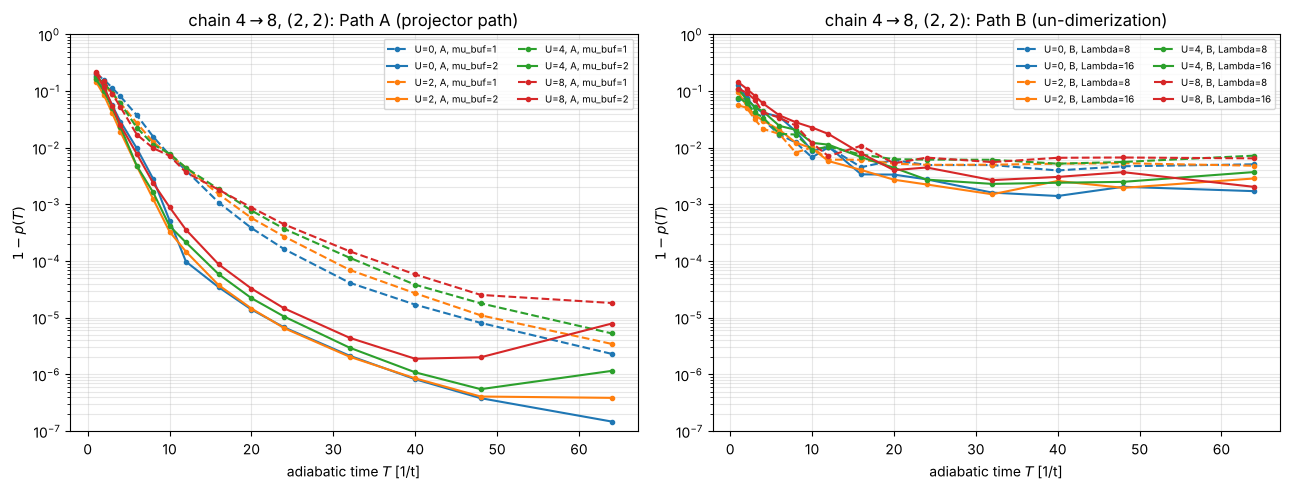
\includegraphics[width=\textwidth]{figs/fig1.png}
  \caption{Refinement of the open chain $4\to8$ at $(2,2)$: $1-p(T)$ along
  Path~A (left; solid $\mu_{\rm buf}=2t$, dashed $\mu_{\rm buf}=t$) and along
  Path~B (right; solid $\Lambda=16t$, dashed $\Lambda=8t$) for $U/t=0,2,4,8$.
  Path~A reaches $1-p<10^{-4}$ by $T=16/t$ at every coupling; Path~B
  saturates at the finite-$\Lambda$ ceiling of a few $10^{-3}$.}
  \label{fig:chain48}
\end{figure*}

\subsection{Which gap controls the refinement: symmetry protection}
\label{sec:symmetry}
Both terms of Eq.~\eqref{eq:pathA} commute with the total spin and with the
point group of the fine lattice (the block structure respects the reflection
of the chain and the $C_{4v}$ group of the square), and the prolongation
maps irreducible representations onto themselves.  The transported state
therefore never leaves the symmetry sector of the coarse ground state --- a
spin singlet, even under reflection, for Table~\ref{tab:chain48} --- and the
states that can be excited along the path are only those of the same sector.
Figure~\ref{fig:weights} makes this explicit: for $U=4t$ the lowest fine
excitations at $0.223t$ (a reflection-odd triplet) and $0.459t$ (an even
triplet) carry weights of order $10^{-31}$, and the first state with nonzero
weight ($4.6\times10^{-5}$), an even singlet, lies at $\Deff=0.588t$; at
$U=8t$ the corresponding numbers are $0.137t$ and $0.286t$ (triplets, zero
weight) and $\Deff=0.366t$.  $\Deff$ falls with $U$ much more slowly than
$\Delta$, which explains the $U$-independent $T^*$.

\begin{figure*}[t]
  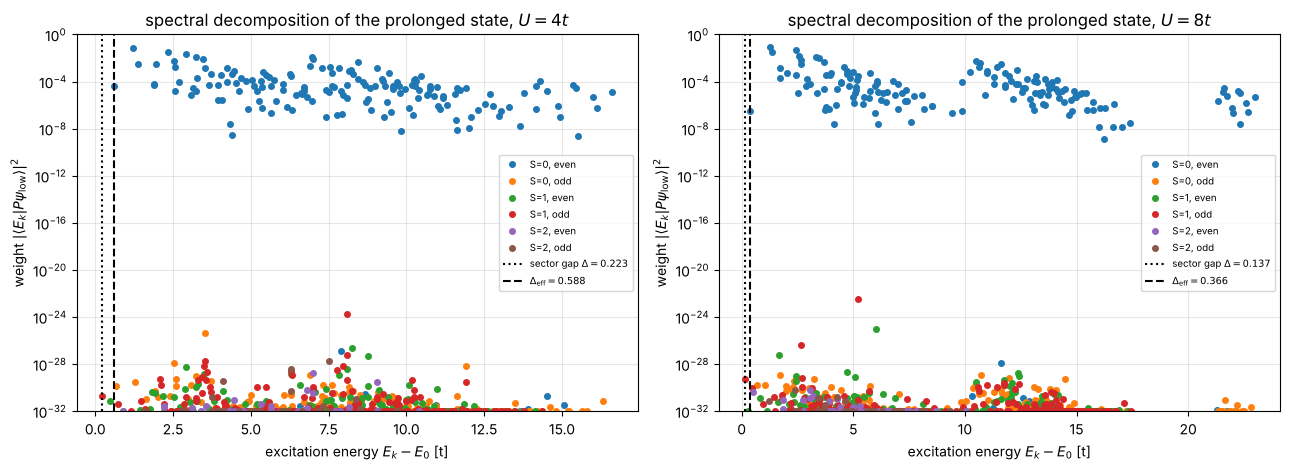
\includegraphics[width=\textwidth]{figs/fig2.png}
  \caption{Spectral decomposition of the prolonged coarse ground state over
  the eigenstates of the eight-site chain at $U=4t$ (left) and $8t$ (right),
  each eigenstate labeled by its total spin and reflection parity.  Only
  even singlets carry weight; the triplets and odd states, including the ones
  that define the sector gap $\Delta$ (dotted), sit at round-off level.  The
  lowest state with weight defines $\Deff$ (dashed).}
  \label{fig:weights}
\end{figure*}

Figure~\ref{fig:gaps} follows the two gaps along Path~A: the sector gap and
the gap to the lowest state with the same $(S,\text{parity})$ as the tracked
state.  The latter never approaches the former; its minimum is $\Deff$
itself, at $s=1$.  This is the isolated-branch condition of the adiabatic
theorem verified numerically along the whole path, within the symmetry
sector in which the transport actually takes place.  The sufficient
adiabatic time of Jansen, Ruskai and Seiler~\cite{Jansen2007}, evaluated as
in paper I once with the sector gap and once with the symmetry-resolved gap,
is smaller by a factor $5$ to $17$ in the second form but remains three to
five orders of magnitude above the empirical $T^*=10/t$ (\SM); the two
numbers answer different questions, a worst-case operator-norm guarantee
for every state in the branch against one overlap for one initial state.
The first-order response norm of the path, $\chi_u(s)$, whose integral sets
the adiabatic leakage at leading order and which paper I obtained in closed
form for the pairing model, is largest at the initial endpoint for every
coupling, $\chi_u(0)=0.38$--$0.87$ for $U/t=0$--$8$, and its modest growth
with $U$ is in line with the flat $T^*$ (\SM).

\begin{figure*}[t]
  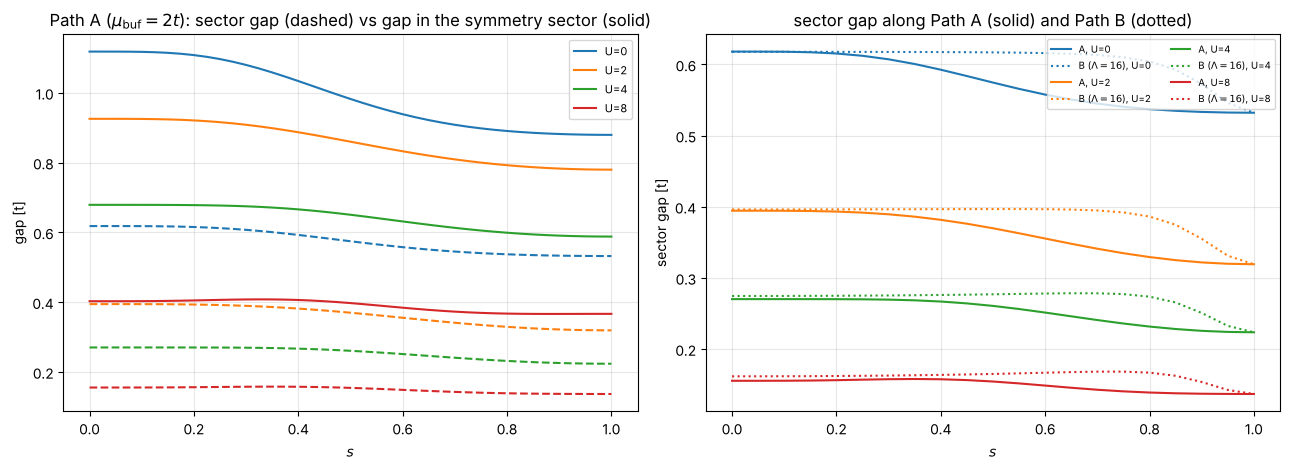
\includegraphics[width=\textwidth]{figs/fig3.png}
  \caption{Left: along Path~A ($\mu_{\rm buf}=2t$), the sector gap (dashed)
  and the gap within the symmetry sector of the tracked state (solid) for
  $U/t=0,2,4,8$.  Right: the sector gap along Path~A (solid) and Path~B with
  $\Lambda=16t$ (dotted); both reach their minimum, the fine-sector gap, at
  $s=1$.}
  \label{fig:gaps}
\end{figure*}

\subsection{The self-similar hierarchy: from the filled dimer to sixteen sites}
\label{sec:dimer}
The self-similarity of Eq.~\eqref{eq:gal1d} allows the chain of refinements
to start from the two-site dimer with $N_\uparrow=N_\downarrow=2$, whose
sector contains a single state --- both sites doubly occupied --- with
$E_{\rm low}=U-4t$: the analog of the $k=2$ determinant that seeded the
$2\to4$ chain of paper I, requiring no classical or variational
preprocessing.  The step $2\to4$ starts from $p_0=0.80$ at $U=0$ down to
$0.48$ at $U=8t$, but with a large effective gap ($\Deff=2.2t$--$0.8t$) it
reaches $p>0.9997$ by $T=16/t$ at every $U$.  Composing steps with the
\emph{refined} four-site state as the input of the $4\to8$ step, and the
shift referenced to its variational energy, the chain $2\to4\to8$ at $U=4t$
with $T=16/t$ per step reaches $p=0.99988$, against $0.99994$ from the exact
coarse input; with $T=8/t$ in the first step the second saturates at
$p=0.9979$, the overlap of its input, because the admixture of other coarse
states refines to other fine states.  The composed chain also beats a
single-shot refinement $2\to8$ with blocks of four ($p_0=0.579$, $p=0.9966$
at $T=16/t$).  The protection survives a doubling of the system: refining
the eight-site chain to sixteen sites at $(2,2)$ ($784\to14\,400$ states,
$U=4t$) starts from $p_0=0.869$, faces a fine-sector gap of only $0.051t$,
and still reaches $p=0.9924$ at $T=8/t$, $0.99931$ at $T=16/t$ and
$0.99995$ at $T=32/t$, because the first state to carry weight lies at
$\Deff=0.138t$ while the eight other states below $0.4t$, including the one
that defines the sector gap, carry none.  Three steps from the filled dimer,
$2\to4\to8\to16$ with $T=16/t$ each and the refined state as the input of
every step, give $p=0.99923$ for the sixteen-site ground state.  The tables
and figures of the dimer step and of the composed chains are in the \SM.

\subsection{Two dimensions: the plaquette and the wrong symmetry sector}
\label{sec:2d}
For the square lattice the first step is $2\times2\to4\times4$.  With one
particle per spin ($16\to256$ states) the refinement behaves as in one
dimension: both ground states are $A_1$, $p_0=0.80$--$0.85$ for $U/t=0,4,8$,
$\Deff\simeq2.1t$--$2.2t$, and $p>0.9997$ at $T=8/t$.  With two particles
per spin ($36\to14\,400$ states) the prolonged coarse ground state has
\emph{zero} overlap with the fine ground state, and the symmetry diagnostics
identify why (Fig.~\ref{fig:2d}).  The half-filled coarse plaquette
(Galerkin parameters $t/2$, $U/4$) has, for every $U>0$, a $B_1$ singlet
ground state with an $A_2$ triplet close above it ($0.071t$ at $U=4t$); the
dilute fine lattice, four electrons on sixteen open sites, has an $A_2$
\emph{triplet} ground state for every $U>0$ studied ($U/t=1$--$8$), the
$B_1$ singlet lying $0.04t$--$0.11t$ above it.  The prolongation commutes
with $\mathbf S^2$ and with $C_{4v}$, so the two cannot be connected: the
fine ground state has weight $0$ on the prolonged coarse ground state,
$0.647$ on the prolonged $A_2$ triplet and $0.007$ on all other coarse
states together ($U=4t$).  Refining that triplet along Path~A
($\mu=E_1^{\rm low}+2t$) reaches $p=0.99944$ at $T=8/t$ and $0.99997$ at
$T=16/t$ although the fine-sector gap is only $0.090t$, since the lowest
state of the $(A_2,S=1)$ sector that carries weight lies $1.77t$ above the
ground state; the same path started from the coarse ground state gives
$p=3\times10^{-27}$.  The lesson for the method is that the state to refine
is the lowest coarse eigenstate \emph{in the symmetry sector of the
target}, which need not be the coarse ground state, that the coarse solver
must be run with the target's quantum numbers imposed or at least
diagnosed, and that the filter cannot rescue a wrong choice, since a state
of zero overlap has nothing to amplify.  Conversely the refinement is a
sensitive detector of a level crossing between the coarse and the fine
problem --- here a singlet--triplet crossing as the filling goes from one
half to one eighth, a property of the filling, not of $U$, over the whole
range studied.  The spectra and the table of the plaquette cases are in
the \SM.

\begin{figure*}[t]
  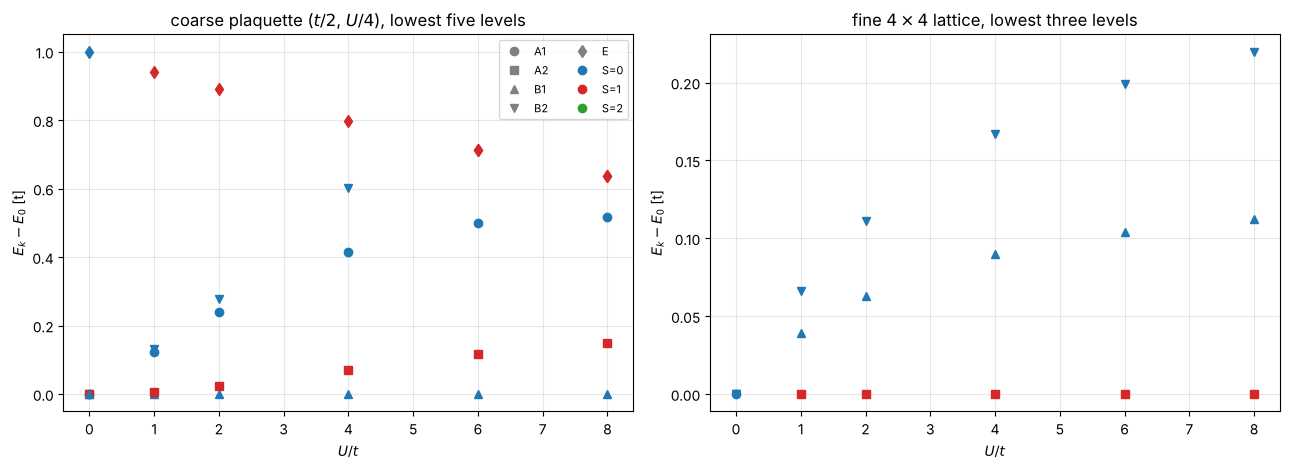
\includegraphics[width=\textwidth]{figs/fig5.png}
  \caption{Lowest levels of the coarse plaquette (left, Galerkin parameters
  $t/2$, $U/4$) and of the fine $4\times4$ lattice (right) at $(2,2)$ versus
  $U/t$, labeled by $C_{4v}$ irrep (marker) and total spin (color).  For
  every $U>0$ the coarse ground state is a $B_1$ singlet and the fine ground
  state an $A_2$ triplet; the prolongation conserves both labels.}
  \label{fig:2d}
\end{figure*}

\subsection{Filtering, and the variational inputs}
\label{sec:res-rodeo}
With $\sigma=5/\Deff$ ($5.7/t$ to $13.6/t$ for $U/t=0$ to $8$) the exact
ensemble filter, Eq.~\eqref{eq:fid}, applied to the prolonged state takes
the infidelity from $1-p_0\simeq0.2$ to $4$--$5\times10^{-3}$ after six
cycles and $2$--$3\times10^{-4}$ after ten, with an acceptance that
converges to $p_0$; applied to the Path-A state refined for $T=16/t$ it
starts from $10^{-4}$ and reaches $0.5$--$1.4\times10^{-6}$ after six
cycles; applied to the eight-site UCCSD state it starts from
$4.7\times10^{-4}$, $3.1\times10^{-3}$ and $1.2\times10^{-2}$ at $U/t=2,4,8$
and reaches $7\times10^{-6}$, $5\times10^{-5}$ and $2\times10^{-4}$
(figure in the \SM).  The refined input converges faster per cycle by the
ratio of the initial infidelities; whether the cycles saved pay for the
refinement gates is the circuit-level question of Sec.~\ref{sec:circuits}.

The variational tables are in the \SM; what matters here is three numbers at
$U=4t$.  The 198-parameter single-layer UCCSD on the eight-site chain
reaches $1-F=3.1\times10^{-3}$ at $3.1\times10^4$ CNOTs; $98$ of its
amplitudes exceed $10^{-3}$, and keeping those ($12$ singles, $86$ doubles)
and re-optimizing gives the same accuracy, $3.145\times10^{-3}$ against
$3.143\times10^{-3}$, at $1.5\times10^4$ CNOTs.  Used as the coarse solver
on the four-site chain, the 26-parameter ansatz ($1-F=3.3\times10^{-3}$)
prolongs with the same $p_0$ as the exact coarse state ($0.800$ against
$0.797$) but the refinement then saturates at $p=0.9967$ instead of
$0.9999$: the coarse stage must be as accurate as the target, or the filter
must do the rest.

% ===========================================================================
\section{Circuits and the matched comparison at eight sites}
\label{sec:circuits}
% ===========================================================================

\subsection{Pauli structure and step costs}
In the block Jordan--Wigner ordering an open chain of $L_f$ sites on $2L_f$
qubits has $4(L_f-1)$ hopping strings $\tfrac t2(X_jX_{j+1}+Y_jY_{j+1})$ of
weight two, $L_f$ interaction strings $\tfrac U4Z_jZ_{j+L_f}$ and $2L_f$
single-$Z$ terms: $52$ strings of weight $\le2$ for $L_f=8$, verified
against the full-space Pauli decomposition on eight qubits, against the
$325$ strings of weight up to eight of the $k=4$ pairing model on half the
qubits.  With the Pauli-rotation primitive of paper I --- $2(w-1)$ CNOTs per
weight-$w$ string, two more per rotation when controlled --- a second-order
Trotter step of the eight-site chain costs $144$ CNOTs and a controlled one
$352$; at sixteen sites, $304$ and $736$.  The product formula groups the
bonds into two layers of disjoint bonds plus the diagonal interaction; each
layer is a product of commuting two-qubit blocks and is realized exactly, so
the Trotter error comes only from the non-commutativity between the three
groups, as on hardware.  The prolongation $4\to8$ costs $16$ CNOTs.  The
embedded coarse term of Path~A is the coarse Hubbard step on the bonding
register ($24$ rotations) with every rotation conditioned on the eight
antibonding qubits being empty: with a clean-ancilla ladder of
relative-phase Toffolis ($6(c-1)+2$ extra CNOTs per rotation) it costs
$1\,088$ CNOTs per application, $7.6$ fine steps, and at sixteen sites
($16$ controls, $48$ rotations) $4\,856$, sixteen fine steps.  Either way
the coarse term, not the fine step, is the cost of Path~A.

\subsection{Trotterized refinement and the baselines}
With second-order product formulas over the groups
$[P(\Hlow-\mu)P^\dagger$ split into its three conditioned coarse groups,
$K_{\rm even},K_{\rm odd},D-\mu]$ for Path~A and
$[(1+\Lambda\cos^2)K_{\rm even},K_{\rm odd},D]$ for Path~B, the exact-slice
overlap at $T=16/t$, $U=4t$ is reproduced to within $10^{-3}$ with
$n_s=128$ steps for Path~A ($p=0.99982$), $256$ for Path~B at $\Lambda=8t$
($0.99213$) and $512$ at $\Lambda=16t$, against $43$ steps for the pairing
path of paper I: the shifted generators have larger norms ($\|B-A\|=14$ for
Path~A, $1+\Lambda$ on the intra-block bonds for Path~B), which makes
$\Lambda=8t$ the better operating point of the two-local path despite its
higher ceiling.  At these step counts the refinement costs
$2.97\times10^5$ CNOTs for Path~A ($2.8\times10^5$ in the coarse term) and
$3.7\times10^4$ for Path~B.  The ramp from the free-fermion determinant
(Givens network $112$ CNOTs) has $p_0=0.7804$ --- essentially the overlap
of the prolonged state, $0.7974$ --- and the same $\Deff=0.588t$, since it
lies in the same symmetry sector; with exact slices it reaches
$p=0.99686$, $0.99960$ and $0.99989$ at $T=8,12,16$, as fast as Path~A and
far above the ceiling of Path~B, and its product-formula version needs
$64$ steps at $T=8/t$ ($9\,328$ CNOTs) and $128$ at $T=16/t$
($0.999659$, $18\,544$ CNOTs).  The step scans are in the \SM.

\subsection{Matched-observable comparison}
\label{sec:budget}
Following Sec.~V.C of paper I we feed the same Trotterized rodeo filter ---
second order, fixed step $\delta t$, $\sigma=5/\Deff=8.5/t$, forty Gaussian
time sets drawn once and shared by all inputs, up to six cycles --- to eight
inputs: the prolonged coarse ground state, the free-fermion determinant,
the pruned and the full UCCSD states, the ramp states at $T=8/t$ and $16/t$,
the Path-B state ($\Lambda=8t$, $n_s=256$) and the Path-A state ($n_s=128$),
and compare the acceptance-weighted ensemble infidelity of the accepted runs
against the CNOTs per attempt and per accepted preparation (input plus
filter, early termination after the first failed ancilla measurement, the
expectation over the time sets).  Two implementation details are forced by
the Hubbard norms.  The fixed step is diagonalized once, so that $n$ steps
are applied exactly and the cycle times are quantized to multiples of
$\delta t$ (on average $68$ steps per cycle, $2.4\times10^4$ CNOTs); the
filter then projects on the eigenvector of the step unitary closest to the
ground state, whose eigenphase is what the energy scan of the rodeo locates
on a device, and we take $\Eobj$ equal to it rather than to $E_0$.  The
Trotter floor of the filter is that eigenvector's infidelity with the exact
ground state: $2.6\times10^{-3}$ at $\delta t=0.25/t$ (the step of paper I,
where $\Eobj-E_0=0.09t$ would also have spoiled the acceptance),
$5.8\times10^{-5}$ at $\delta t=0.1/t$ and $3.5\times10^{-6}$ at $0.05/t$;
we operate at $\delta t=0.1/t$, where $\Eobj-E_0=0.013t$.  Because the cycle
times are quantized every cycle shares the eigenvectors of the step
unitary, so the long-run state of the filter is that eigenvector itself
and, with $\Eobj$ on its eigenphase, the acceptance tends to the input's
weight on it instead of decaying --- the fixed-step analog of the averaged
post-selection map of paper I.  The sampled infidelities carry bootstrap
relative standard errors of up to $18\%$ for the unrefined inputs at $M=6$
and below $10\%$ for the refined and variational ones.

\begin{table*}[t]
  \caption{Matched-observable comparison for the chain $4\to8$ at $U=4t$:
  the same Trotterized rodeo filter (second order, $\delta t=0.1/t$,
  $\sigma=8.5/t$, $\Eobj$ the Trotter-effective ground energy, forty time
  sets) applied to every input.  $p$ is the overlap of the input and
  ``prep'' its CNOT count (prolongation $16$; Givens network $112$;
  refinement or ramp $n_s$ second-order steps of $144$ CNOTs, plus
  $2\times1\,088$ per step for the coarse term of Path~A; UCCSD pruned
  $15\,120$, full $30\,864$); $M=0$ is the unfiltered input.  For $M=2$ and
  $6$ cycles: the ensemble infidelity (bootstrap relative standard error in
  parentheses), the cumulative acceptance $P$, and the CNOTs per accepted
  preparation (input plus filter, early termination; the CNOTs per attempt
  are $P$ times smaller).}
  \label{tab:budget}
  \centering\scriptsize
  \setlength{\tabcolsep}{2.5pt}
  \begin{tabular}{lcc|c|ccc|ccc}
  \toprule
  input & $p$ & prep & $M=0$ & \multicolumn{3}{c|}{$M=2$} & \multicolumn{3}{c}{$M=6$}\\
  & & & $1-\mathcal F$ & $1-\mathcal F$ & $P$ & CNOTs & $1-\mathcal F$ & $P$ & CNOTs\\
  \midrule
  prolonged & 0.7974 & 16 & $2.0{\times}10^{-1}$ & $6.0{\times}10^{-2}$ (7\%) & 0.848 & $5.2{\times}10^{4}$ & $4.7{\times}10^{-3}$ (18\%) & 0.802 & $1.5{\times}10^{5}$\\
  determinant & 0.7804 & 112 & $2.2{\times}10^{-1}$ & $6.6{\times}10^{-2}$ (5\%) & 0.831 & $5.3{\times}10^{4}$ & $5.0{\times}10^{-3}$ (17\%) & 0.779 & $1.6{\times}10^{5}$\\
  UCCSD pruned (98) & 0.9969 & 15\,120 & $3.1{\times}10^{-3}$ & $8.2{\times}10^{-4}$ (6\%) & 0.997 & $6.2{\times}10^{4}$ & $1.1{\times}10^{-4}$ (7\%) & 0.997 & $1.6{\times}10^{5}$\\
  UCCSD full (198) & 0.9969 & 30\,864 & $3.1{\times}10^{-3}$ & $8.1{\times}10^{-4}$ (6\%) & 0.997 & $7.8{\times}10^{4}$ & $1.1{\times}10^{-4}$ (7\%) & 0.997 & $1.7{\times}10^{5}$\\
  ramp, $T=8$, $n_s=64$ & 0.9969 & 9\,328 & $3.1{\times}10^{-3}$ & $7.8{\times}10^{-4}$ (14\%) & 0.998 & $5.6{\times}10^{4}$ & $8.9{\times}10^{-5}$ (10\%) & 0.997 & $1.5{\times}10^{5}$\\
  ramp, $T=16$, $n_s=128$ & 0.9997 & 18\,544 & $3.4{\times}10^{-4}$ & $1.3{\times}10^{-4}$ (6\%) & 1.000 & $6.5{\times}10^{4}$ & $6.2{\times}10^{-5}$ (3\%) & 1.000 & $1.6{\times}10^{5}$\\
  Path B ($\Lambda=8t$), $n_s=256$ & 0.9921 & 36\,880 & $7.9{\times}10^{-3}$ & $2.0{\times}10^{-3}$ (6\%) & 0.994 & $8.4{\times}10^{4}$ & $2.0{\times}10^{-4}$ (9\%) & 0.992 & $1.8{\times}10^{5}$\\
  Path A (split), $n_s=128$ & 0.9998 & 296\,976 & $1.8{\times}10^{-4}$ & $9.1{\times}10^{-5}$ (2\%) & 1.000 & $3.4{\times}10^{5}$ & $6.0{\times}10^{-5}$ (1\%) & 1.000 & $4.4{\times}10^{5}$\\
  \bottomrule
  \end{tabular}
\end{table*}

\begin{figure*}[t]
  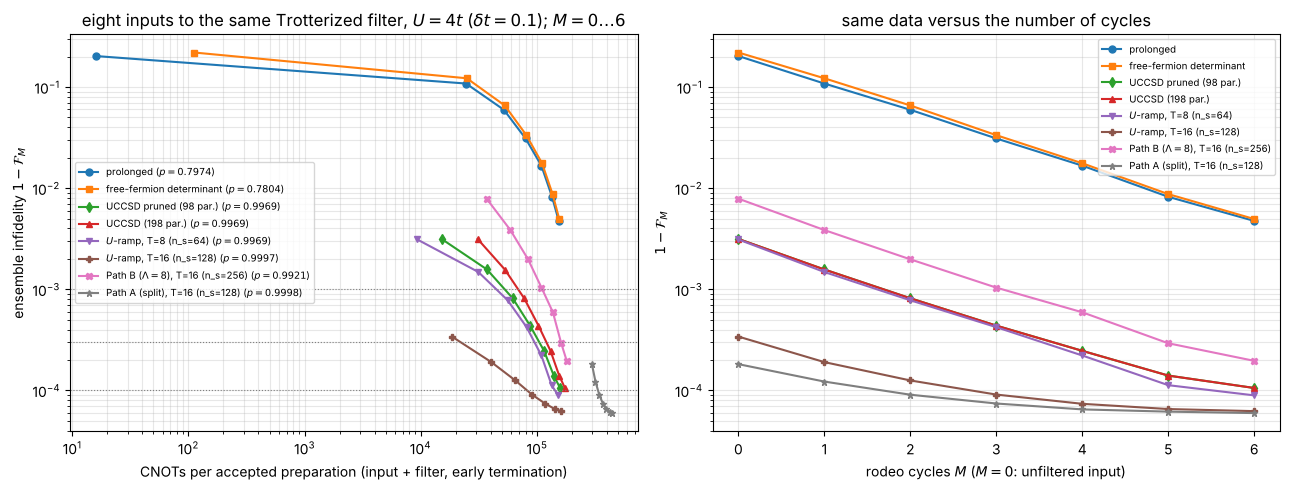
\includegraphics[width=\textwidth]{figs/fig10.png}
  \caption{Cost versus accuracy for the chain $4\to8$ at $U=4t$: ensemble
  infidelity against CNOTs per accepted preparation (left; the first point
  of each curve, $M=0$, is the unfiltered input, dotted lines the targets
  $10^{-3}$, $3\times10^{-4}$, $10^{-4}$) and against the number of cycles
  (right) for the eight inputs of Table~\ref{tab:budget}, all cleaned by the
  same Trotterized filter.  The refined inputs reach the Trotter floor of
  $5.8\times10^{-5}$ within six cycles; the unrefined ones do not.}
  \label{fig:budget}
\end{figure*}

Table~\ref{tab:budget} and Fig.~\ref{fig:budget} give the verdict at eight
sites; the operating points (minimum cost at each target, with the cycle
count that attains it) are tabulated in the \SM.  At every target the
cheapest route is the ramp from the free-fermion determinant at $T=16/t$:
$1.9\times10^4$ CNOTs for $10^{-3}$ without any filter cycle,
$4.0\times10^4$ for $3\times10^{-4}$ with one cycle and $9.1\times10^4$ for
$10^{-4}$ with three.  The pruned UCCSD state costs $3.3$ and $2.9$ times
more at the first two targets and does not reach $10^{-4}$ within six
cycles; the full pool is a further $10$--$25\%$ more expensive.  Path~B at
$\Lambda=8t$ costs $7.4$ and $4$ times the ramp, because its preparation is
twice as expensive and starts twenty times worse owing to the ceiling.
Path~A delivers the best unfiltered input ($1-p=1.8\times10^{-4}$) but at
$3\times10^5$ CNOTs, sixteen times the ramp; it is the only input other than
the ramp to reach $10^{-4}$, at $3.4\times10^5$ CNOTs.  The prolonged state
and the bare determinant need six cycles and $1.5$--$1.6\times10^5$ CNOTs to
reach $5\times10^{-3}$ and reach none of the targets.  Only the inputs that
start within a decade of the floor converge to it within six cycles; the
floor is set by $\delta t$, but whether it is reached is set by the input.
The costs are per accepted preparation at the operating point of each input;
the setup costs --- the classical optimization and its measurements for the
variational states, the calibration of $(T,\mu_{\rm buf},n_s)$ for the
adiabatic inputs, the energy scan that locates $\Eobj$ --- are not included
and are amortized over the preparations that use them, and the refinement
parameters are the first grid values that meet the accuracy criterion, not
optimized ones; a joint search may move every curve by a factor of order
unity, but not the factor sixteen of the conditioned coarse term nor the
twenty-fold ceiling of Path~B.

% ===========================================================================
\section{Eight to sixteen sites at the circuit level}
\label{sec:large}
% ===========================================================================
The comparison of Sec.~\ref{sec:budget} is at one size, where the
free-fermion determinant has the same overlap and the same $\Deff$ as the
prolonged coarse eigenstate; the case for refinement rests on the regime
where the coarse eigenstate is the better start.  Here the chain $8\to16$
at $(2,2)$, $U=4t$ ($784\to14\,400$ states, thirty-two qubits) is taken to
the circuit level with the same accounting.  Every product-formula factor
of the fine chain is applied through the Kronecker structure of
Eq.~\eqref{eq:kron} as a pair of $120\times120$ exponentials, the embedded
coarse term of Path~A exactly through the $784$-dimensional coarse space,
and the variational comparators with sparse generators; the
Trotter-effective ground state of the fixed-step filter, which cannot be
obtained by diagonalizing the $14\,400$-dimensional step unitary, is
obtained by iterating the quantized-time filter itself from the exact
ground state (details and validation against the dense eight-site machinery
in the \SM).

\paragraph{The inputs.}
The prolonged coarse ground state now starts ahead of the determinant,
$p_0=0.869$ against $0.716$, with the same $\Deff=0.138t$ for both (the
determinant lies in the same symmetry sector), while the sector gap is
$0.051t$ and the sector gap along the ramp falls from $0.165t$ to $0.051t$.
Figure~\ref{fig:large}(left) shows the exact-slice transports.  The ramp
needs $T=32/t$ for $1-p=4.1\times10^{-3}$ and $T=64/t$ for $8.1\times10^{-4}$
($1.1\times10^{-3}$ at $48/t$), against $T=8/t$ for $p=0.9924$
($T^*=16/t$, $p=0.99931$; $0.99995$ at $32/t$) along Path~A with
$\mu_{\rm buf}=2t$; a larger shift does not help at this
size ($p(16)=0.99879$ and $0.99792$ at $\mu_{\rm buf}=4t$ and $8t$), because
it raises the norm of the generator without widening a gap that is already
set by $\Deff$.  Path~B sits at its ceiling from $T=16/t$ on, $p=0.99492$ and $0.99531$
at $T=16/t$ and $32/t$ for $\Lambda=8t$ ($0.99500$ and $0.99605$ for
$\Lambda=16t$), the same few $10^{-3}$ as at eight sites.  The product
formulas need $n_s=128$ second-order steps for the ramp at $T=16/t$
($p=0.96927$, $39\,392$ CNOTs) and $256$ at $T=32/t$ ($0.99556$, $78\,304$
CNOTs; with $32$ steps, $\delta t=1/t$, the ramp overlap collapses to
$0.005$), $256$ for Path~B at $\Lambda=8t$, $T=16/t$ ($0.99476$, $77\,856$
CNOTs plus the coarse preparation); Path~A at
$T=16/t$ with the coarse term split into its conditioned groups reaches
$p=0.99835$ at $n_s=128$ for $1.28\times10^6$ CNOTs, of which
$1.24\times10^6$ in the coarse term, while at $T=8/t$ the product formula
plateaus at $p=0.99079$ from $n_s=128$ on, $1.6\times10^{-3}$ below the
exact-slice value, so that the shorter path cannot be made to reproduce its
exact transport at any step count.  The single-layer UCCSD ansatz on
sixteen sites has $1\,022$ parameters, costs $3.4\times10^5$ CNOTs and
reaches only $1-F=7.0\times10^{-3}$ (against $3.1\times10^{-3}$ with $198$
parameters at eight sites); pruning to the $255$ amplitudes above
$10^{-3}$ keeps that accuracy at $8.8\times10^4$ CNOTs.
Figure~\ref{fig:large}(right) shows ADAPT-VQE with the same pool: at eight
sites the adaptive ansatz passes the single-layer accuracy at $66$
operators and reaches $10^{-3}$ at $149$ and $3\times10^{-4}$ at $194$
operators (a third of the template's operators, chosen adaptively and
with repeats, do what the full template does); at sixteen sites it
needs $187$ operators ($6.8\times10^4$ CNOTs) to reach $10^{-2}$ and has
not reached $3\times10^{-3}$ after $200$.  The convergence is slow because
the ground state spreads over many small amplitudes rather than a few large
ones, the opposite of the pairing case of paper I, where five operators
sufficed at eight qubits; and, unlike there, the adaptive ansatz does not
undercut the ramp even at eight sites, where the $149$-operator state
($2.3\times10^4$ CNOTs) fed to the filter of Sec.~\ref{sec:budget} reaches
$10^{-3}$, $3\times10^{-4}$ and $10^{-4}$ at $2.3\times10^4$,
$6.9\times10^4$ and $1.5\times10^5$ CNOTs against the ramp's
$1.9\times10^4$, $4.0\times10^4$ and $9.1\times10^4$.

\begin{figure*}[t]
  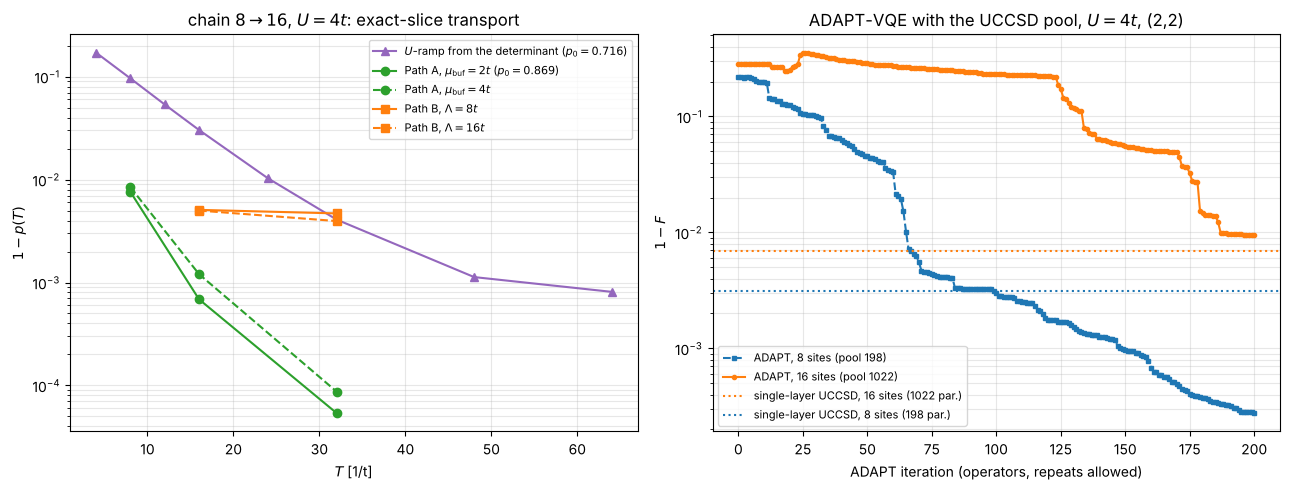
\includegraphics[width=\textwidth]{figs/fig11.png}
  \caption{The chain $8\to16$ at $(2,2)$, $U=4t$.  Left: $1-p(T)$ with exact
  slices for the ramp from the free-fermion determinant, Path~A with
  $\mu_{\rm buf}=2t$ and $4t$ and Path~B with $\Lambda=8t$ and $16t$.  Right:
  ADAPT-VQE with the UCCSD pool at eight and at sixteen sites, infidelity
  against the number of operators, with the single-layer UCCSD values as
  horizontal lines.}
  \label{fig:large}
\end{figure*}

\paragraph{The filter at thirty-two qubits.}
With $\sigma=5/\Deff=36/t$ and $\delta t=0.1/t$ a cycle takes $289$ steps on
average, $2.1\times10^5$ CNOTs, nine times the cycle of
Sec.~\ref{sec:budget}: $4.3$ times more steps, since $\Deff$ is $4.3$ times
smaller, and $2.1$ times more per step.  The Trotter-effective ground
energy lies $4.9\times10^{-3}t$ above $E_0$ and the floor of the filter is
$3.7\times10^{-5}$.  The cost of the filter therefore scales as
$1/\Deff$ per cycle at fixed $\delta t$, and an input that is cheap but
needs several cycles pays this price in full at every size.

\paragraph{Matched comparison.}
Table~\ref{tab:large} and Fig.~\ref{fig:largebudget} feed eight inputs to
this filter with twenty shared time sets: the determinant, the prolonged
coarse ground state, the pruned UCCSD state, the ramp at $T=16/t$ and
$32/t$, Path~B ($\Lambda=8t$, $T=16/t$), Path~A ($T=16/t$) and the ADAPT
state at its first iteration below $10^{-2}$; every input that starts from
the coarse eigenstate is charged, in addition, its preparation by the
cheapest eight-site route of Table~\ref{tab:budget} that reaches
$3\times10^{-4}$, the ramp at $T=16/t$ ($18\,544$ CNOTs).  The floor is
reached by none of the inputs within six cycles (the best, Path~A, is at
$7.4\times10^{-5}$, twice the floor); the bootstrap relative standard errors
reach $20$--$35\%$ at $M=6$ with twenty time sets, and the operating points
below are read with that uncertainty.  The ramp at $T=32/t$ is the cheapest
route at every target: $7.8\times10^4$ CNOTs for $10^{-2}$ without a
cycle, $3.0\times10^5$ for $3\times10^{-3}$ with one, $7.9\times10^5$ for
$10^{-3}$ with three and $1.3\times10^6$ for $3\times10^{-4}$ with five.
Path~B is within $1$--$6\%$ of it at the three tighter targets, a tie
within the sampling error, and $23\%$ above it at $10^{-2}$, where only the
preparation counts: its preparation ($9.6\times10^4$ CNOTs including the
coarse eigenstate) and its starting infidelity ($5.2\times10^{-3}$ against
$4.4\times10^{-3}$) match the ramp's, so at this size the coarse eigenstate
transported along the cheapest path is as good a start as the determinant
transported for twice the time.  The variational routes cost $1.3$--$1.9$
times more at $3\times10^{-3}$ and $10^{-3}$ --- the adaptive state at
$10^{-2}$ is the cheapest unfiltered input ($6.8\times10^4$ CNOTs) but then
needs four cycles for $10^{-3}$ --- and come within $1$--$13\%$ of the
ramp only at $3\times10^{-4}$, where every input needs five or six cycles
and the preparation no longer matters.  Path~A delivers the best unfiltered input,
$1.7\times10^{-3}$, and reaches $10^{-3}$ with one cycle and
$3\times10^{-4}$ with three, at $1.9$ and $1.6$ times the cost of the ramp:
the factor sixteen of eight sites has become a factor two, because the
ramp itself now needs three cycles, $6.4\times10^5$ CNOTs of filtering,
before it reaches $10^{-3}$, while the $1.2\times10^6$ CNOTs of the
conditioned coarse term buy a start that needs one.  The ramp at $T=16/t$, the cheapest input
at eight sites, needs six cycles for $10^{-3}$ here and is beaten by the
two-local path and by both variational inputs, and the prolonged state and the determinant
reach $2.4\times10^{-3}$ and $7.1\times10^{-3}$ after six cycles, with
acceptances $0.87$ and $0.72$.

\begin{table*}[t]
  \caption{Matched comparison for the chain $8\to16$ at $U=4t$ (thirty-two
  qubits): the same Trotterized rodeo filter (second order,
  $\delta t=0.1/t$, $\sigma=36/t$, $\Eobj$ the Trotter-effective ground
  energy, twenty time sets) applied to every input.  ``prep'' counts the
  Givens network ($480$ CNOTs), the prolongation ($32$), the second-order
  steps ($304$ CNOTs, plus $2\times4\,856$ per step for the coarse term of
  Path~A), the variational circuits, and, for every input that starts from
  the coarse eigenstate, its preparation by the cheapest eight-site route
  of Table~\ref{tab:budget} that reaches $3\times10^{-4}$ ($18\,544$ CNOTs).
  $1-\mathcal F$ at $M=0$ (the unfiltered input) and after six cycles
  (bootstrap relative standard error in parentheses; the cumulative
  acceptance after six cycles equals $p$ to two digits for every input);
  then the minimum CNOTs per accepted preparation at each
  target infidelity, with the cycle count in parentheses (a dash: not
  reached within six cycles).  The full $M=0$--$6$ data are in the \SM.}
  \label{tab:large}
  \centering\scriptsize
  \setlength{\tabcolsep}{2pt}
  \begin{tabular}{lcc|cc|cccc}
  \toprule
  input & $p$ & prep & $1-\mathcal F_0$ & $1-\mathcal F_6$ & $10^{-2}$ & $3{\times}10^{-3}$ & $10^{-3}$ & $3{\times}10^{-4}$\\
  \midrule
  determinant & 0.7162 & 480 & $2.8{\times}10^{-1}$ & $7.1{\times}10^{-3}$ (18\%) & $1.5{\times}10^{6}$ (6) & --- & --- & ---\\
  prolonged & 0.8692 & 18\,576 & $1.3{\times}10^{-1}$ & $2.4{\times}10^{-3}$ (13\%) & $1.3{\times}10^{6}$ (5) & $1.4{\times}10^{6}$ (6) & --- & ---\\
  UCCSD pruned (255) & 0.9930 & 87\,776 & $7.0{\times}10^{-3}$ & $1.3{\times}10^{-4}$ (12\%) & $8.8{\times}10^{4}$ (0) & $5.6{\times}10^{5}$ (2) & $1.1{\times}10^{6}$ (4) & $1.3{\times}10^{6}$ (5)\\
  ADAPT (187 op.) & 0.9901 & 68\,008 & $9.9{\times}10^{-3}$ & $1.7{\times}10^{-4}$ (11\%) & $6.8{\times}10^{4}$ (0) & $5.4{\times}10^{5}$ (2) & $1.0{\times}10^{6}$ (4) & $1.4{\times}10^{6}$ (6)\\
  ramp, $T{=}16$, $n_s{=}128$ & 0.9693 & 39\,392 & $3.1{\times}10^{-2}$ & $4.2{\times}10^{-4}$ (35\%) & $5.2{\times}10^{5}$ (2) & $1.0{\times}10^{6}$ (4) & $1.4{\times}10^{6}$ (6) & ---\\
  ramp, $T{=}32$, $n_s{=}256$ & 0.9956 & 78\,304 & $4.4{\times}10^{-3}$ & $8.6{\times}10^{-5}$ (23\%) & $7.8{\times}10^{4}$ (0) & $3.0{\times}10^{5}$ (1) & $7.9{\times}10^{5}$ (3) & $1.3{\times}10^{6}$ (5)\\
  Path B ($\Lambda{=}8t$), $T{=}16$, $n_s{=}256$ & 0.9948 & 96\,400 & $5.2{\times}10^{-3}$ & $1.4{\times}10^{-4}$ (13\%) & $9.6{\times}10^{4}$ (0) & $3.2{\times}10^{5}$ (1) & $8.1{\times}10^{5}$ (3) & $1.3{\times}10^{6}$ (5)\\
  Path A (split), $T{=}16$, $n_s{=}128$ & 0.9983 & 1\,300\,624 & $1.7{\times}10^{-3}$ & $7.4{\times}10^{-5}$ (17\%) & $1.3{\times}10^{6}$ (0) & $1.3{\times}10^{6}$ (0) & $1.5{\times}10^{6}$ (1) & $2.0{\times}10^{6}$ (3)\\
  \bottomrule
  \end{tabular}
\end{table*}

\begin{figure*}[t]
  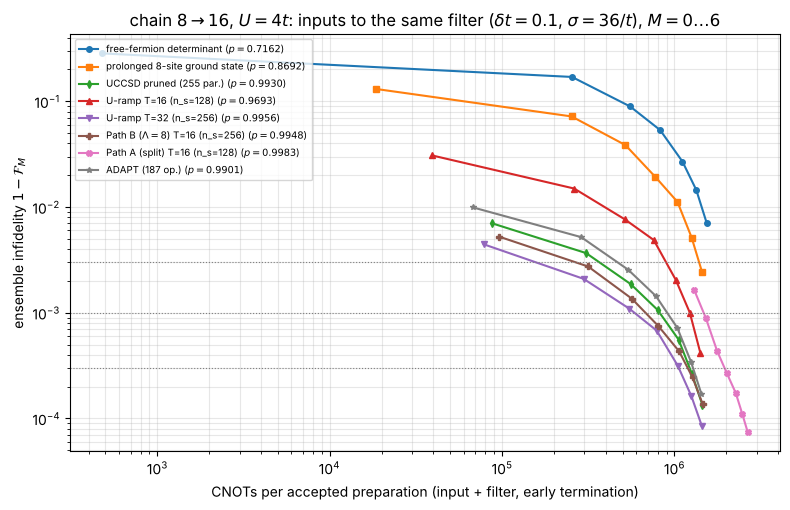
\includegraphics[width=0.75\textwidth]{figs/fig12.png}
  \caption{Cost versus accuracy for the chain $8\to16$ at $U=4t$: ensemble
  infidelity against CNOTs per accepted preparation ($M=0\ldots6$) for the
  inputs of Table~\ref{tab:large}, all cleaned by the same Trotterized
  filter; dotted lines mark $3\times10^{-3}$, $10^{-3}$ and $3\times10^{-4}$.}
  \label{fig:largebudget}
\end{figure*}

% ===========================================================================
\section{Discussion}
\label{sec:discussion}
% ===========================================================================
\paragraph{What the benchmark shows.}
At sixteen qubits the ordinary adiabatic ramp from the free-fermion
determinant is the cheapest route to every target accuracy, by a factor of
three over the pruned variational ansatz, four to seven over the two-local
refinement path and sixteen over the projector path, for a reason specific
to the size: the determinant has the same overlap and the same
symmetry-protected gap as the prolonged coarse eigenstate, so the ramp
starts from the same place, travels at the same speed and pays only for
fine-chain steps.  At thirty-two qubits the premise changes --- the coarse
eigenstate starts ahead, the ramp needs twice the time, the single-layer
ansatz has lost two orders of magnitude and the adaptive ansatz barely
reaches $10^{-2}$ with two hundred operators --- and the margins collapse:
the two-local refinement path ties with the ramp from $3\times10^{-3}$
down, the variational routes cost $1.3$--$1.9$ times more, and the projector
path costs twice the ramp instead of sixteen times.  The ramp is still the
cheapest, but the comparison is now decided by the filter cycles each
input needs, at $2\times10^5$ CNOTs per cycle, not by the preparation
--- and the input that needs fewest is the refined one.  The trend from
eight to sixteen sites is therefore the one the refinement proposal
predicted: as the free-fermion overlap decays, the coarse eigenstate
becomes the better start, and the open question is no longer whether the
refinement stage can pay but whether its transport can be compiled without
the conditioned coarse term --- Path~B, whose ceiling of a few $10^{-3}$ is
what keeps it from inheriting the $1.7\times10^{-3}$ start of Path~A at a
fifteenth of the cost.  Two lessons are
inherited from paper I and sharpened.  A conditioned coarse term is never
affordable: at sixteen sites it costs sixteen fine steps per application,
and the two-local path or a schedule that avoids the embedding altogether
is the only form of the projector path worth compiling.  And the figure of
merit is the cost at fixed accuracy per accepted preparation with the
filter cycles included, where the cycle cost grows as $1/\Deff$: at fixed
cycle count every input ``converges to the floor'' only in the sense that
the best ones do.

\paragraph{Which gap matters.}
The quantity that controls the refinement is the symmetry-protected
effective gap $\Deff$, not the sector gap; this is why $T^*$ is flat in $U$
and in size, why the sufficient time of the adiabatic theorem is a closer
(though still remote) estimate when evaluated with the symmetry-resolved
gap, and why $\Deff$ is the right width for the filter.  Paper I found that
its scan of the refinement time against the shift-controlled gap did not
identify a power law; the lesson here is that any such scan must be made
against the gap in the symmetry sector of the tracked state, with the
response norm held fixed, before an exponent can be read off.  The
zero-overlap plaquette is the converse and a warning for any refinement,
fusion or nucleation scheme: the coarse state must carry the quantum
numbers of the target, which the ED diagnostics of Sec.~\ref{sec:model}
--- or, on a device, measurements of $\mathbf S^2$ and of the point-group
characters --- can check before any gate is spent.

\paragraph{Lattice versus basis refinement, and coarse accuracy.}
The lattice refinement is structurally cleaner than the basis refinement
of paper I: a Galerkin coarse model in closed form, a self-similar
hierarchy that starts from a single basis state, a two-local Hamiltonian
with $O(L_f)$ Pauli strings of weight two, a prolongation of $O(N_c)$ gates.
Against this stand the conditioned coarse term, Path~B as its two-local
replacement with a $(t/\Lambda)^2$ ceiling and a step count that grows with
$\Lambda$, and three to ten times more Trotter steps than the pairing path
for the same adiabatic time, because the shifted generators have larger
norms.  Composing steps with refined inputs and starting from a variational
coarse state show the same ceiling: an admixture of other coarse
eigenstates refines to other fine eigenstates and caps the final overlap at
roughly the input fidelity, so the coarse stage must be as accurate as the
target, or the filter must pay for the difference; the filled dimer, which
is exact, is from this point of view the best coarse state the hierarchy
has.

\paragraph{Outlook.}
At fixed $U/t$ the hierarchy is self-similar, so refinement does not by
itself reach strong coupling; a path that raises $U$ with the resolution,
or a refinement at fixed filling, are the options.  In one dimension the
dimer-seeded hierarchy and the nucleation of a chain from a
dimer~\cite{Sadia2026} start from the same state and reach the same target
by refining resolution versus growing the domain, and the Hubbard chain is
the natural place to compare the two at matched gate count; the optimized
variants of either (a warm-started variational path) are the obvious way to
cut the $10^2$--$10^3$ Trotter steps found here.  The refinement and filter
parameters are calibrated against the exact answer; a device-level protocol
(an energy scan for $\Eobj$, acceptance statistics for $\sigma$ and
$\delta t$, a convergence test in $T$ and $n_s$ on the measured energy) and
a comparison at matched shot budget including the training measurements of
the variational routes are the missing pieces for a hardware run, for which
the $4\to8$ chain and the $(1,1)$ plaquette (thirty-two qubits,
$256$-dimensional sector) are within reach of current devices.

\section*{Acknowledgments}
The work of C.G. and G.L. acknowledges funding from the European Union's
Horizon Europe research and innovation program under the Marie
Sk\l{}odowska-Curie Grant Agreement No.\ 101126636.  M.H.-J. is partially
supported by U.S. National Science Foundation (NSF) Grants PHY-1404159 and
PHY-2310020.  The authors acknowledge Anthropic's Claude for assistance with
literature search and coding.

\section*{Code and data availability}
\label{sec:code}
All results are produced by the notebook
\texttt{notebooks/ResolutionRefHubbard.ipynb}, built by
\texttt{scripts/build\_notebook\_hubbard.py} on the module
\texttt{pairinglib.hubbard} (lattices, sector ED, block prolongation,
Galerkin coarse model, both paths, exact and Trotterized refinement, the
ensemble rodeo formula and its Trotterized version, the symmetry
diagnostics, the sector-level UCCSD and ADAPT-VQE, the Kronecker-structured
product formulas of the sixteen-site study and the gate counting), which is
covered by the test suite of the repository~\cite{Code}; the figures are
extracted from the executed notebook, and the \SM{} and the notebook
together document every number quoted.  The ED reference code (Hubbard and
$t$--$J$ models; chain, square and checkerboard lattices) is the notebook
\texttt{Hubbard.ipynb}~\cite{HubbardNotebook}, whose conventions the module
follows.

% ===========================================================================
\begin{thebibliography}{99}
\bibitem{Peruzzo2014} A.~Peruzzo, J.~McClean, P.~Shadbolt, M.-H.~Yung,
X.-Q.~Zhou, P.~J.~Love, A.~Aspuru-Guzik, and J.~L.~O'Brien, Nat.\ Commun.\
\textbf{5}, 4213 (2014).
\bibitem{McClean2018} J.~R.~McClean, S.~Boixo, V.~N.~Smelyanskiy, R.~Babbush,
and H.~Neven, Nat.\ Commun.\ \textbf{9}, 4812 (2018).
\bibitem{Albash2018} T.~Albash and D.~A.~Lidar, Rev.\ Mod.\ Phys.\ \textbf{90},
015002 (2018).
\bibitem{Choi2021} K.~Choi, D.~Lee, J.~Bonitati, Z.~Qian, and J.~Watkins,
Phys.\ Rev.\ Lett.\ \textbf{127}, 040505 (2021).
\bibitem{Qian2024} Z.~Qian \emph{et al.}, Eur.\ Phys.\ J.\ A \textbf{60}, 151 (2024).
\bibitem{Bogner2026} S.~Bogner, H.~Hergert, M.~Hjorth-Jensen, R.~LaRose,
D.~Lee, and M.~Patkowski, ``Quantum state preparation with resolution
refinement,'' Phys.\ Lett.\ B \textbf{875}, 140363 (2026); arXiv:2511.14732.
\bibitem{EigenQPairing2026} S.~Bogner, C.~Glittum, H.~Hergert,
M.~Hjorth-Jensen, G.~Lange, R.~LaRose, D.~Lee, F.~P.~Massel, and J.~P.~Sadia,
``Resolution refinement followed by the rodeo algorithm: a gate-level
benchmark of eigenstate-preparation routes on the pairing Hamiltonian,''
submitted to Phys.\ Rev.\ C (2026).
\bibitem{Hubbard1963} J.~Hubbard, Proc.\ R.\ Soc.\ London A \textbf{276}, 238 (1963).
\bibitem{Arovas2022} D.~P.~Arovas, E.~Berg, S.~A.~Kivelson, and S.~Raghu,
Annu.\ Rev.\ Condens.\ Matter Phys.\ \textbf{13}, 239 (2022).
\bibitem{Wecker2015} D.~Wecker, M.~B.~Hastings, N.~Wiebe, B.~K.~Clark,
C.~Nayak, and M.~Troyer, Phys.\ Rev.\ A \textbf{92}, 062318 (2015).
\bibitem{Cade2020} C.~Cade, L.~Mineh, A.~Montanaro, and S.~Stanisic,
Phys.\ Rev.\ B \textbf{102}, 235122 (2020).
\bibitem{Cai2020} Z.~Cai, Phys.\ Rev.\ Applied \textbf{14}, 014059 (2020).
\bibitem{Stanisic2022} S.~Stanisic \emph{et al.}, Nat.\ Commun.\ \textbf{13}, 5743 (2022).
\bibitem{Cohen2023} T.~D.~Cohen and H.~Oh, Phys.\ Rev.\ A \textbf{108}, 032422 (2023).
\bibitem{BeeLindgren2022} M.~Bee-Lindgren, Z.~Qian, M.~DeCross, N.~C.~Brown,
C.~N.~Gilbreth, J.~Watkins, X.~Zhang, and D.~Lee, arXiv:2208.13557 (2022).
\bibitem{Patkowski2025fusion} M.~Patkowski, O.~Ayyildiz, M.~Kebri\v{c},
K.~L.~C.~Hunt, and D.~Lee, ``Hierarchical fusion method for scalable quantum
eigenstate preparation,'' Phys.\ Rev.\ A \textbf{113}, 052442 (2026);
arXiv:2510.19039.
\bibitem{Sadia2026} J.~P.~Sadia, M.~Hjorth-Jensen, D.~Lee, and R.~LaRose,
``Digital quantum state preparation by nucleation,'' arXiv:2609.37527 (2026).
\bibitem{Code} Repository \texttt{pairing-eigenq}, [URL to be inserted];
archived version: Zenodo, [DOI to be inserted].
\bibitem{Grimsley2019} H.~R.~Grimsley, S.~E.~Economou, E.~Barnes, and
N.~J.~Mayhall, Nat.\ Commun.\ \textbf{10}, 3007 (2019).
\bibitem{SM} See Supplemental Material at [URL will be inserted by
publisher] for the adiabatic bound and the response norm of the path, the
dimer-seeded hierarchy and the composition of steps, the plaquette spectra,
the variational tables, the Trotterized refinement at eight sites, the
exact-ensemble filter, the ingredients and validation of the thirty-two-qubit
study, and the operating-point tables.
\bibitem{Jansen2007} S.~Jansen, M.-B.~Ruskai, and R.~Seiler, J.~Math.\ Phys.\
\textbf{48}, 102111 (2007).
\bibitem{HubbardNotebook} \todo{Authors}, ``The Hubbard and $t$--$J$ models:
exact diagonalization on chain, square and checkerboard lattices,''
\texttt{paper3/Hubbard.ipynb} (2026).
\end{thebibliography}

\end{document}
